\documentclass{article}\usepackage[]{graphicx}\usepackage[]{color}
%% maxwidth is the original width if it is less than linewidth
%% otherwise use linewidth (to make sure the graphics do not exceed the margin)
\makeatletter
\def\maxwidth{ %
  \ifdim\Gin@nat@width>\linewidth
    \linewidth
  \else
    \Gin@nat@width
  \fi
}
\makeatother

\definecolor{fgcolor}{rgb}{0.345, 0.345, 0.345}
\newcommand{\hlnum}[1]{\textcolor[rgb]{0.686,0.059,0.569}{#1}}%
\newcommand{\hlstr}[1]{\textcolor[rgb]{0.192,0.494,0.8}{#1}}%
\newcommand{\hlcom}[1]{\textcolor[rgb]{0.678,0.584,0.686}{\textit{#1}}}%
\newcommand{\hlopt}[1]{\textcolor[rgb]{0,0,0}{#1}}%
\newcommand{\hlstd}[1]{\textcolor[rgb]{0.345,0.345,0.345}{#1}}%
\newcommand{\hlkwa}[1]{\textcolor[rgb]{0.161,0.373,0.58}{\textbf{#1}}}%
\newcommand{\hlkwb}[1]{\textcolor[rgb]{0.69,0.353,0.396}{#1}}%
\newcommand{\hlkwc}[1]{\textcolor[rgb]{0.333,0.667,0.333}{#1}}%
\newcommand{\hlkwd}[1]{\textcolor[rgb]{0.737,0.353,0.396}{\textbf{#1}}}%
\let\hlipl\hlkwb

\usepackage{framed}
\makeatletter
\newenvironment{kframe}{%
 \def\at@end@of@kframe{}%
 \ifinner\ifhmode%
  \def\at@end@of@kframe{\end{minipage}}%
  \begin{minipage}{\columnwidth}%
 \fi\fi%
 \def\FrameCommand##1{\hskip\@totalleftmargin \hskip-\fboxsep
 \colorbox{shadecolor}{##1}\hskip-\fboxsep
     % There is no \\@totalrightmargin, so:
     \hskip-\linewidth \hskip-\@totalleftmargin \hskip\columnwidth}%
 \MakeFramed {\advance\hsize-\width
   \@totalleftmargin\z@ \linewidth\hsize
   \@setminipage}}%
 {\par\unskip\endMakeFramed%
 \at@end@of@kframe}
\makeatother

\definecolor{shadecolor}{rgb}{.97, .97, .97}
\definecolor{messagecolor}{rgb}{0, 0, 0}
\definecolor{warningcolor}{rgb}{1, 0, 1}
\definecolor{errorcolor}{rgb}{1, 0, 0}
\newenvironment{knitrout}{}{} % an empty environment to be redefined in TeX

\usepackage{alltt}

\usepackage{polyglossia}
  \setmainlanguage{spanish}
\usepackage{fontspec}
\usepackage{geometry}
\usepackage{parskip}
\usepackage{amsmath}
\usepackage{booktabs}
\usepackage[backend=bibtex,style=authoryear,citestyle=authoryear,doi=false,isbn=false,url=false]{biblatex}
%  \addbibresource{NER-bib.bib}
\usepackage{hyperref}

\newcommand*{\eng}[1]{\textsl{#1}}
\newcommand*{\paq}[1]{\textbf{#1}}

% Code chunk



\title{Notas de Econometría en R}
\author{Alvaro Carril\thanks{Estas notas son un intento de condensar lo justo y necesario para poder seguir un curso de econometría con R.
Luego de recopilar material de muchas clases y ayudantías de econometría, en general pensadas para ser aplicadas en Stata, decidí que podía intentar hacer estas clases en R y usar esta guía como material de apoyo.
Mi prioridad fue ser breve y conciso, por lo que estas notas no son un buen comienzo para aprender R (o econometría); son un complemento.
Si hay algún error o quieres hacer algún comentario, mi correo es \texttt{acarril@fen.uchile.cl}.}}
\IfFileExists{upquote.sty}{\usepackage{upquote}}{}
\begin{document}

\maketitle
\tableofcontents

\clearpage

\section{Introducción}

\subsection{Qué es R}

R es un ambiente de software y un lenguaje de programación interpretado para hacer análisis estadístico y gráficos. Es una implementación de S, un lenguaje de programación matemático orientado a objetos más antiguo. Es software libre y de código abierto, activamente usado y ampliado por estadísticos y colaboradores de otras disciplinas.

R es mucho más flexible que la mayoría de los paquetes estadísticos normalmente usados por economistas. Es un lenguaje de programación completamente desarrollado, no sólo un programa con tests y métodos pre-programados.


\subsection{Obtener R}

La instalación base de R puede obtenerse de \url{https://www.r-project.org/}. Una vez instalado puedes usar RGui para usarlo. Sin embargo, usualmente yo tomo dos pasos adicionales para obtener más flexibilidad. El primero es instalar RStudio, un IDE para R que incluye una consola, editor con resaltado de sintaxis, historial de comandos y varias otras vainas que lo hacen más útil que RGui, especialmente si eres principiante. Puedes descargar RStudio de \url{https://www.rstudio.com/}, y también es gratis.

Finalmente, a mi me gusta poder interactuar con R desde la línea de comandos, igual que puedo hacer con Python o Julia. Para poder hacer esto en Windows tenemos que ejecutar R:

\begin{knitrout}
\definecolor{shadecolor}{rgb}{0.969, 0.969, 0.969}\color{fgcolor}\begin{kframe}
\begin{alltt}
\hlstr{"C:\textbackslash{}Program Files\textbackslash{}R\textbackslash{}R-3.4.0\textbackslash{}bin\textbackslash{}x64\textbackslash{}R"}
\end{alltt}
\end{kframe}
\end{knitrout}

Obviamente, tienes que reemplazar este directorio por el que corresponde a tu instalación. 

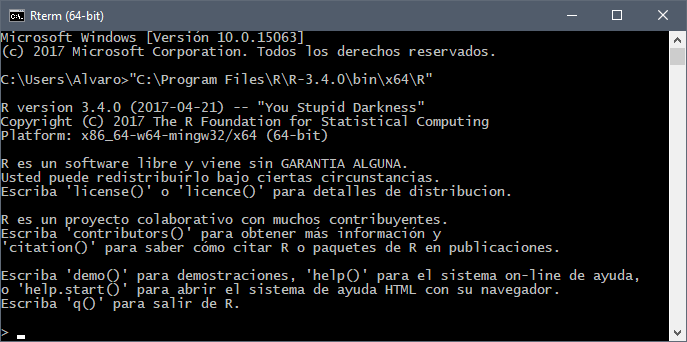
\includegraphics[width=\linewidth]{sss/r-win-command-prompt}

\subsection{Usar R interactivamente y a través de scripts}

\begin{knitrout}
\definecolor{shadecolor}{rgb}{0.969, 0.969, 0.969}\color{fgcolor}\begin{kframe}
\begin{alltt}
\hlkwd{getwd}\hlstd{()}
\end{alltt}
\begin{verbatim}
## [1] "/Users/alvaro/Dropbox (Personal)/Proyectos/NER"
\end{verbatim}
\end{kframe}
\end{knitrout}



\section{Trabajando con datos}

\subsection{Objetos y asignaciones}

R es un lenguaje interpretado, lo que significa que ejecuta nuestras instrucciones directamente, sin compilar un programa previo. Podemos usar R interactivamente a través de la consola:
\begin{knitrout}
\definecolor{shadecolor}{rgb}{0.969, 0.969, 0.969}\color{fgcolor}\begin{kframe}
\begin{alltt}
\hlnum{1}\hlopt{+}\hlnum{2}
\end{alltt}
\begin{verbatim}
## [1] 3
\end{verbatim}
\end{kframe}
\end{knitrout}

La mayoría de las operaciones y funciones en R no guardan el resultado de su ejecución. Por ejemplo, el resultado anterior (\verb|3|) es calculado pero no puede ser reutilizado sin volverse a calcular. Para lograr esto tenemos que asignar el resultado de la operación a un objeto:
\begin{knitrout}
\definecolor{shadecolor}{rgb}{0.969, 0.969, 0.969}\color{fgcolor}\begin{kframe}
\begin{alltt}
\hlstd{x} \hlkwb{<-} \hlnum{1}\hlopt{+}\hlnum{2}
\end{alltt}
\end{kframe}
\end{knitrout}



\section{Regresión lineal}

El modelo de regresión lineal es el caballo de batalla de la econometría aplicada.
En su forma más simple usualmente se escribe como
\begin{equation}
y_i = \beta_0 + \beta_1 x_i + \mu_i.
\end{equation}
donde $i = 1, \ldots, n$ es un índice que identifica a las observaciones (filas) en los datos. Podríamos tener $n$ personas, familias o empresas. Suponemos que la variable dependiente $y$ es una función lineal de la variable independiente, $x$.

Por ejemplo, podríamos tener un vector $y$ con los salarios de $n$ personas y modelarlo como una función lineal de los años de educación de esas personas, $x$. Resulta útil tener una base de datos concreta con estos vectores, por lo que usaremos 

\begin{knitrout}
\definecolor{shadecolor}{rgb}{0.969, 0.969, 0.969}\color{fgcolor}\begin{kframe}
\begin{alltt}
\hlkwd{library}\hlstd{(modelr)}
\hlstd{sim1}
\end{alltt}
\begin{verbatim}
## # A tibble: 30 x 2
##        x         y
##    <int>     <dbl>
##  1     1  4.199913
##  2     1  7.510634
##  3     1  2.125473
##  4     2  8.988857
##  5     2 10.243105
##  6     2 11.296823
##  7     3  7.356365
##  8     3 10.505349
##  9     3 10.511601
## 10     4 12.434589
## # ... with 20 more rows
\end{verbatim}
\end{kframe}
\end{knitrout}

El comando \verb|library(modelr)| carga el paquete \paq{modelr}. Este paquete incluye la base de datos \verb|sim1|, que contiene datos simulados. Al escribir \verb|sim1| imprimimos el encabezado de la base de datos. Vemos que la base tiene 30 observaciones ($n=30$).

Podemos graficar estos datos usando \paq{ggplot2}, un paquete muy poderoso para crear gráficos. Lo cargamos y luego creamos un gráfico de puntos con los datos:

\begin{knitrout}
\definecolor{shadecolor}{rgb}{0.969, 0.969, 0.969}\color{fgcolor}\begin{kframe}
\begin{alltt}
\hlkwd{library}\hlstd{(ggplot2)}
\hlkwd{ggplot}\hlstd{(sim1,} \hlkwd{aes}\hlstd{(x, y))} \hlopt{+} \hlkwd{geom_point}\hlstd{()}
\end{alltt}
\end{kframe}

{\centering \includegraphics[width=4in,height=3in]{figure/unnamed-chunk-6-1} 

}



\end{knitrout}

Vemos que existe una evidente relación lineal entre $x$ e $y$: a mayor nivel de educaci

Primero que nada conviene imprimir el encabezado de la base de datos, que corresponde a las primeras observaciones.

\begin{knitrout}
\definecolor{shadecolor}{rgb}{0.969, 0.969, 0.969}\color{fgcolor}\begin{kframe}
\begin{alltt}
\hlstd{sim1}
\end{alltt}
\begin{verbatim}
## # A tibble: 30 x 2
##        x         y
##    <int>     <dbl>
##  1     1  4.199913
##  2     1  7.510634
##  3     1  2.125473
##  4     2  8.988857
##  5     2 10.243105
##  6     2 11.296823
##  7     3  7.356365
##  8     3 10.505349
##  9     3 10.511601
## 10     4 12.434589
## # ... with 20 more rows
\end{verbatim}
\end{kframe}
\end{knitrout}

Esto es lo primero que debieses hacer antes de empezar a utilizar datos nuevos, ya que permite tener una idea rápida sobre ellos. Vemos que hay 30 observaciones ($n=30$) y que \verb|x| solo toma valores enteros (y hay valores repetidos), mientras que \verb|y| es continua.

\hrulefill

El modelo de regresión lineal es el caballo de batalla de la econometría aplicada, y puede escribirse como
\begin{equation}
y_i = x_i^T \beta + \epsilon_i,
\end{equation}
donde $i = 1, \ldots, n$ es un índice que identifica a las observaciones (filas) en los datos. Podríamos tener $n$ personas, familias o empresas.
También es común escribir el mismo modelo en forma matricial:
\begin{equation}
y = X \beta + \epsilon.
\end{equation}

En estas ecuaciones $y$ (o $y_i$) es un vector $n \times 1$ que representa la variable dependiente del modelo, es decir, la variable que queremos explicar. Por ejemplo, $y$ podría ser un vector de salario cuyos valores son los ingresos mensuales de $n$ personas.
La variable dependiente es explicada por un conjunto de $k$ variables independientes, usalmente denotadas por $X$. Entonces $X$ es una matriz $n\times k$, ya que contiene información de $k$ variables (columnas) para $n$ observaciones (filas).

Al estimar este tipo de modelos usualmente nos interesa determinar $\beta$, que representa la relación lineal entre $y$ y $X$, es decir, entre la variable dependiente y el conjunto de variables independientes que la explican. El vector $\beta$ contiene $k \times 1$ coeficientes de regresión, de forma que estimaremos un coeficiente por cada variable incluída en $X$.
Finalmente $\epsilon$ es el llamado término de error, un vector $n \times 1$ que captura las discrepancias para cada observación $i$ que resulta de imponer una relación lineal entre $X$ e $y$.

Para entender bien todo esto resulta muy útil manipular un modelo simple. Para esto usaremos \verb|sim1|, una base de datos simulada que contiene dos variables: \verb|x| e \verb|y|. Cargamos el paquete \paq{modelr} para poder acceder esta base de datos, y además cargamos \paq{ggplot2} para crear gráficos:

\begin{knitrout}
\definecolor{shadecolor}{rgb}{0.969, 0.969, 0.969}\color{fgcolor}\begin{kframe}
\begin{alltt}
\hlkwd{library}\hlstd{(modelr)}
\hlkwd{library}\hlstd{(ggplot2)}
\end{alltt}
\end{kframe}
\end{knitrout}

Primero que nada conviene imprimir el encabezado de la base de datos, que corresponde a las primeras observaciones.

\begin{knitrout}
\definecolor{shadecolor}{rgb}{0.969, 0.969, 0.969}\color{fgcolor}\begin{kframe}
\begin{alltt}
\hlstd{sim1}
\end{alltt}
\begin{verbatim}
## # A tibble: 30 x 2
##        x         y
##    <int>     <dbl>
##  1     1  4.199913
##  2     1  7.510634
##  3     1  2.125473
##  4     2  8.988857
##  5     2 10.243105
##  6     2 11.296823
##  7     3  7.356365
##  8     3 10.505349
##  9     3 10.511601
## 10     4 12.434589
## # ... with 20 more rows
\end{verbatim}
\end{kframe}
\end{knitrout}

Esto es lo primero que debieses hacer antes de empezar a utilizar datos nuevos, ya que permite tener una idea rápida sobre ellos. Vemos que hay 30 observaciones ($n=30$) y que \verb|x| solo toma valores enteros (y hay valores repetidos), mientras que \verb|y| es continua.

Ahora graficamos estos datos para hacernos una idea de la relación que existe entre ambos:

\begin{knitrout}
\definecolor{shadecolor}{rgb}{0.969, 0.969, 0.969}\color{fgcolor}\begin{kframe}
\begin{alltt}
\hlkwd{ggplot}\hlstd{(sim1,} \hlkwd{aes}\hlstd{(x, y))} \hlopt{+} \hlkwd{geom_point}\hlstd{()}
\end{alltt}
\end{kframe}

{\centering \includegraphics[width=4in,height=3in]{figure/unnamed-chunk-10-1} 

}



\end{knitrout}

Oh sorpresa, los datos simulados presentan una clara correlación positiva. Parece casi diseñado para ser modelado linealmente...
%La pregunta relevante, sin embargo, es cuál línea usar.
Recordemos que en este caso nuestro modelo lineal puede escribirse simplemente como

\begin{equation*}
y_i = \beta_0 + \beta_1 x_i + \epsilon_i 
\end{equation*}

Entonces la pregunta relevante es ``¿qué línea es la que mejor captura la relación entre $x$ e $y$?''.
Notemos que en este caso bidimensional simple $\beta_0$ y $\beta_1$ representan el intercepto y la pendiente de la recta, respectivamente.
Por lo tanto la pregunta también puede plantearse como: ¿cuáles son los valores de $\beta_0$ y $\beta_1$ que describen mejor esta relación?


\begin{knitrout}
\definecolor{shadecolor}{rgb}{0.969, 0.969, 0.969}\color{fgcolor}

{\centering \includegraphics[width=4in,height=3in]{figure/unnamed-chunk-11-1} 

}



\end{knitrout}

\subsection{Mínimos Cuadrados Ordinarios}

El método de Mínimos Cuadrados Ordinarios (MCO) es una respuesta directa a la pregunta que planteamos recién: ¿qué criterio conviene usar para elegir el modelo lineal que se ajuste ``mejor'' a los datos?
Lo que propone MCO es minimizar la suma de los errores al cuadrado.
Geométricamente, esto equivale a minimizar la distancia vertical entre los puntos y la recta definida por el modelo.

\begin{knitrout}
\definecolor{shadecolor}{rgb}{0.969, 0.969, 0.969}\color{fgcolor}

{\centering \includegraphics[width=4in,height=3in]{figure/unnamed-chunk-12-1} 

}



\end{knitrout}

La distancia entre un puntos y la recta el error de predicción del modelo, capturado por $\epsilon_i$. Es decir que para cada observación $i$ tenemos una medida de la magnitud del error que esta elección de $\beta_0$ y $\beta_1$ produce. El criterio de MCO entonces es elegir $\beta_0$ y $\beta_1$ tal que se minimice el promedio de todos los errores al cuadrado.\footnote{¿Por qué al cuadrado? Porque se asume que es irrelevante si el error es una subestimación o una sobreestimación, de forma que lo único que importa es la magnitud. ¿Por qué no se usa el valor absoluto entonces? Buena pregunta.}



\hrulefill
%Para esta sección usaremos el paquete \paq{AER}, que incluye varias bases de datos para econometría. Ahora usaremos \verb|AER::CPS1988|, que contiene información de salarios de EE.UU. en Marzo de 1988.

\begin{knitrout}
\definecolor{shadecolor}{rgb}{0.969, 0.969, 0.969}\color{fgcolor}\begin{kframe}
\begin{alltt}
\hlkwd{library}\hlstd{(AER)}
\hlkwd{data}\hlstd{(}\hlstr{"CPS1988"}\hlstd{)}
\end{alltt}
\end{kframe}
\end{knitrout}

Consideremos la vieja y confiable ecuación de salarios de Mincer:

\begin{equation}
\text{salario}_i = \beta_0 + \beta_1 \text{educación}_i + \beta_2 \text{experiencia}_i + \epsilon_i
\label{eq:mincer}
\end{equation}

En términos de la base \verb|CPS1988|, nos interesan por el momento las variables \verb|wage|, \verb|education| y \verb|experience|. Podemos estimar este modelo lineal simple escribiendo

\begin{knitrout}
\definecolor{shadecolor}{rgb}{0.969, 0.969, 0.969}\color{fgcolor}\begin{kframe}
\begin{alltt}
\hlkwd{lm}\hlstd{(wage} \hlopt{~} \hlstd{education} \hlopt{+} \hlstd{experience,} \hlkwc{data} \hlstd{= CPS1988)}
\end{alltt}
\begin{verbatim}
## 
## Call:
## lm(formula = wage ~ education + experience, data = CPS1988)
## 
## Coefficients:
## (Intercept)    education   experience  
##     -385.08        60.90        10.61
\end{verbatim}
\end{kframe}
\end{knitrout}

El resultado que imprime \verb|lm()| es una versión muy abreviada de todo lo que fue calculado, ya que sólo entrega las estimaciones de los coeficientes $\beta$ del modelo. Para ver más detalles podemos guardar los resultados de \verb|lm()| en el objeto \verb|mincer| y luego aplicarle la función \verb|summary()|:

\begin{knitrout}
\definecolor{shadecolor}{rgb}{0.969, 0.969, 0.969}\color{fgcolor}\begin{kframe}
\begin{alltt}
\hlstd{mincer} \hlkwb{<-} \hlkwd{lm}\hlstd{(wage} \hlopt{~} \hlstd{education} \hlopt{+} \hlstd{experience,} \hlkwc{data} \hlstd{= CPS1988)}
\hlkwd{summary}\hlstd{(mincer)}
\end{alltt}
\begin{verbatim}
## 
## Call:
## lm(formula = wage ~ education + experience, data = CPS1988)
## 
## Residuals:
##     Min      1Q  Median      3Q     Max 
## -1136.1  -220.8   -48.3   154.5 18156.1 
## 
## Coefficients:
##              Estimate Std. Error t value Pr(>|t|)    
## (Intercept) -385.0834    13.2428  -29.08   <2e-16 ***
## education     60.8964     0.8828   68.98   <2e-16 ***
## experience    10.6057     0.1957   54.19   <2e-16 ***
## ---
## Signif. codes:  0 '***' 0.001 '**' 0.01 '*' 0.05 '.' 0.1 ' ' 1
## 
## Residual standard error: 411.5 on 28152 degrees of freedom
## Multiple R-squared:  0.1768,	Adjusted R-squared:  0.1768 
## F-statistic:  3024 on 2 and 28152 DF,  p-value: < 2.2e-16
\end{verbatim}
\end{kframe}
\end{knitrout}

Normalmente se usa la función \verb|summary()| en objetos de datos, tales comos vectores o marcos de datos, para obtener estadística descriptiva del objeto (promedio, desviación estándar, etc.). Al usarla en un objeto con resultados de una estimación ---como en este caso--- nos entregará información importantes de dicha estimación, como el $R^2$ del modelo o los errores estándar de los coeficientes.

Podemos extraer otro tipo de información y objetos del modelo. La función \verb|residuals()| entrega los residuos del modelo, y \verb|vcov()| entrega la matriz de varianzas-covarianzas de los coeficientes:

\begin{knitrout}
\definecolor{shadecolor}{rgb}{0.969, 0.969, 0.969}\color{fgcolor}\begin{kframe}
\begin{alltt}
\hlcom{# Residuos}
\hlkwd{residuals}\hlstd{(mincer)}
\hlcom{# Matriz de varianzas-covarianzas:}
\hlkwd{vcov}\hlstd{(mincer)}
\end{alltt}
\end{kframe}
\end{knitrout}

Obviamente estas funciones sólo sirven para realizar otras computaciones y no para ser impresas directamente, y es por eso que he omitido su resultado.

Es común querer estimar un modelo sin intercepto, lo que se logra escribiendo el intercepto explícitamente en la fórmula, usualmente como 0:

\begin{knitrout}
\definecolor{shadecolor}{rgb}{0.969, 0.969, 0.969}\color{fgcolor}\begin{kframe}
\begin{alltt}
\hlkwd{lm}\hlstd{(wage} \hlopt{~} \hlnum{0} \hlopt{+} \hlstd{education} \hlopt{+} \hlstd{experience,} \hlkwc{data} \hlstd{= CPS1988)}
\end{alltt}
\begin{verbatim}
## 
## Call:
## lm(formula = wage ~ 0 + education + experience, data = CPS1988)
## 
## Coefficients:
##  education  experience  
##     36.551       7.653
\end{verbatim}
\end{kframe}
\end{knitrout}

Podemos especificar formas funcionales más complejas para nuestro modelo básico expresado en \eqref{eq:mincer}, incluyendo términos interactuados con \verb|*| y términos cuadráticos encerrados en la función \verb|I()|:

\begin{knitrout}
\definecolor{shadecolor}{rgb}{0.969, 0.969, 0.969}\color{fgcolor}\begin{kframe}
\begin{alltt}
\hlkwd{lm}\hlstd{(wage} \hlopt{~} \hlstd{experience} \hlopt{+} \hlkwd{I}\hlstd{(experience}\hlopt{^}\hlnum{2}\hlstd{)} \hlopt{+} \hlstd{education} \hlopt{+} \hlstd{education}\hlopt{*}\hlstd{parttime,}
   \hlstd{CPS1988)}
\end{alltt}
\begin{verbatim}
## 
## Call:
## lm(formula = wage ~ experience + I(experience^2) + education + 
##     education * parttime, data = CPS1988)
## 
## Coefficients:
##           (Intercept)             experience        I(experience^2)  
##             -432.9424                27.3992                -0.3992  
##             education            parttimeyes  education:parttimeyes  
##               58.3777               167.0709               -33.8042
\end{verbatim}
\end{kframe}
\end{knitrout}

También es posible aplicar a los vectores alguna transformación directamente, como el logaritmo o raíz cuadrada (con \verb|log()| y \verb|sqrt()|). Hay que ser cuidados con los valores que toman las variables a las que se aplican estas funciones, recordando que la raíz cuadrada no está definida para números negativos y que $\ln(0) \rightarrow -\infty$:

\begin{knitrout}
\definecolor{shadecolor}{rgb}{0.969, 0.969, 0.969}\color{fgcolor}\begin{kframe}
\begin{alltt}
\hlkwd{sqrt}\hlstd{(}\hlopt{-}\hlnum{1}\hlstd{)}
\end{alltt}
\begin{verbatim}
## [1] NaN
\end{verbatim}
\begin{alltt}
\hlkwd{log}\hlstd{(}\hlnum{0}\hlstd{)}
\end{alltt}
\begin{verbatim}
## [1] -Inf
\end{verbatim}
\end{kframe}
\end{knitrout}


\subsection{Extraer y calcular información de una regresión}

Un objeto de clase \verb|lm| ---como \verb|mincer|--- es una lista que contiene varios atributos. Estos atributos son objetos calculados por \verb|lm()| con información a la que podemos acceder. Para imprimir una lista completa de los atributos de un objeto usamos \verb|attributes()|:

\begin{knitrout}
\definecolor{shadecolor}{rgb}{0.969, 0.969, 0.969}\color{fgcolor}\begin{kframe}
\begin{alltt}
\hlkwd{attributes}\hlstd{(mincer)}
\end{alltt}
\begin{verbatim}
## $names
##  [1] "coefficients"  "residuals"     "effects"       "rank"         
##  [5] "fitted.values" "assign"        "qr"            "df.residual"  
##  [9] "xlevels"       "call"          "terms"         "model"        
## 
## $class
## [1] "lm"
\end{verbatim}
\end{kframe}
\end{knitrout}

Para usar algún atributo necesitamos la notación de signo \verb|$|. Por ejemplo, podemos guardar el vector $\hat y$ con

\begin{knitrout}
\definecolor{shadecolor}{rgb}{0.969, 0.969, 0.969}\color{fgcolor}\begin{kframe}
\begin{alltt}
\hlstd{yhat} \hlkwb{<-} \hlstd{mincer}\hlopt{$}\hlstd{fitted.values}
\end{alltt}
\end{kframe}
\end{knitrout}

Esto puede ser útil, por ejemplo, al implementar el método de variables instrumentales en dos etapas, donde tenemos que rescatar los valores estimados $\hat x$ en la primera etapa para luego incluirlos en la ecuación original. Escribiendo \verb|?lm| puedes obtener más información sobre todos estos atributos.

Vimos que \verb|summary()| calcula e imprime otra información útil del resultado de una regresión. Análogo a \verb|lm()|, \verb|summary()| también tiene atributos a los que podemos acceder:

\begin{knitrout}
\definecolor{shadecolor}{rgb}{0.969, 0.969, 0.969}\color{fgcolor}\begin{kframe}
\begin{alltt}
\hlstd{mincer.summ} \hlkwb{<-} \hlkwd{summary}\hlstd{(mincer)}
\hlkwd{attributes}\hlstd{(mincer.summ)}
\end{alltt}
\begin{verbatim}
## $names
##  [1] "call"          "terms"         "residuals"     "coefficients" 
##  [5] "aliased"       "sigma"         "df"            "r.squared"    
##  [9] "adj.r.squared" "fstatistic"    "cov.unscaled" 
## 
## $class
## [1] "summary.lm"
\end{verbatim}
\end{kframe}
\end{knitrout}

Usando estos atributos podemos calcular fácilmente algunos resultados útiles. Por ejemplo, podemos obtener la matriz de varianzas-covarianzas del modelo:

\begin{knitrout}
\definecolor{shadecolor}{rgb}{0.969, 0.969, 0.969}\color{fgcolor}\begin{kframe}
\begin{alltt}
\hlstd{(mincer.summ}\hlopt{$}\hlstd{sigma)}\hlopt{^}\hlnum{2} \hlopt{*} \hlstd{mincer.summ}\hlopt{$}\hlstd{cov.unscaled}
\end{alltt}
\begin{verbatim}
##             (Intercept)    education  experience
## (Intercept)  175.370845 -11.08702313 -1.34464546
## education    -11.087023   0.77941945  0.04954238
## experience    -1.344645   0.04954238  0.03830960
\end{verbatim}
\end{kframe}
\end{knitrout}

Finalmente, además de los cálculos que podemos efectuar directamente con estos atributos, existen muchas funciones que toman un objeto de clase \verb|lm| y calculan directamente algún resultado. Por ejemplo, podríamos haber calculado la matriz de varianzas-covarianzas directamente con \verb|vcov()|:

\begin{knitrout}
\definecolor{shadecolor}{rgb}{0.969, 0.969, 0.969}\color{fgcolor}\begin{kframe}
\begin{alltt}
\hlkwd{vcov}\hlstd{(mincer)}
\end{alltt}
\begin{verbatim}
##             (Intercept)    education  experience
## (Intercept)  175.370845 -11.08702313 -1.34464546
## education    -11.087023   0.77941945  0.04954238
## experience    -1.344645   0.04954238  0.03830960
\end{verbatim}
\end{kframe}
\end{knitrout}

Otras funciones útiles para usar con este tipo de objetos son:

\begin{knitrout}
\definecolor{shadecolor}{rgb}{0.969, 0.969, 0.969}\color{fgcolor}\begin{kframe}
\begin{alltt}
\hlcom{# Calcular suma de los cuadrados de los residuos (SSR):}
\hlkwd{deviance}\hlstd{(mincer)}
\hlcom{# Extraer log-likelihood (LL):}
\hlkwd{logLik}\hlstd{(mincer)} \hlcom{# no tiene mucho sentido aquí porque no estimamos con MV}
\hlcom{# Calcular el critero de información de Akaike (AIC):}
\hlkwd{AIC}\hlstd{(mincer)}
\end{alltt}
\end{kframe}
\end{knitrout}

Notar que \verb|AIC()| define el criterio como
\begin{equation}
AIC = -2 \ln \widehat L(p) + K\cdot 2,
\end{equation}
donde $K$ es el número de parámetros estimados y $\widehat L(p)$ es la función de verosimilitud. En muchos casos se prefiere que el criterio sea $AIC/N$, es decir, usar el Criterio de Información Bayesiano (BIC). Esto es,
\begin{equation}
BIC = -2 \ln \widehat L(p) + K \cdot \ln N,
\end{equation}
donde $N$ es el número de observaciones.
Para calcular el BIC también usamos \verb|AIC()|, pero especificando un parámetro de penalización distinto:
\begin{knitrout}
\definecolor{shadecolor}{rgb}{0.969, 0.969, 0.969}\color{fgcolor}\begin{kframe}
\begin{alltt}
\hlkwd{AIC}\hlstd{(mincer,} \hlkwc{k} \hlstd{=} \hlkwd{log}\hlstd{(}\hlkwd{NROW}\hlstd{(CPS1988)))} \hlcom{# fijar k=2 es igual que el AIC clásico}
\end{alltt}
\begin{verbatim}
## [1] 418915.2
\end{verbatim}
\end{kframe}
\end{knitrout}


\subsection{Heterocedasticidad}

La heterocedasticidad es un problema que es más difícil de pronunciar que de entender: ocurre cuando la dispersión de la variable dependiente es cambiante para distintos valores de la variable independiente. Podemos generar fácilmente un conjunto de datos para visualizar el problema:

\begin{knitrout}
\definecolor{shadecolor}{rgb}{0.969, 0.969, 0.969}\color{fgcolor}\begin{kframe}
\begin{alltt}
\hlkwd{set.seed}\hlstd{(}\hlnum{314}\hlstd{)}
\hlstd{n} \hlkwb{<-} \hlnum{256}                           \hlcom{# Número de observaciones}
\hlstd{x} \hlkwb{<-} \hlstd{(}\hlnum{1}\hlopt{:}\hlstd{n)}\hlopt{/}\hlstd{n}                       \hlcom{# Valores de `x`}
\hlstd{e} \hlkwb{<-} \hlkwd{rnorm}\hlstd{(n,} \hlkwc{sd}\hlstd{=}\hlnum{1}\hlstd{)}                \hlcom{# Valores aleatorios de una normal}
\hlstd{i} \hlkwb{<-} \hlkwd{order}\hlstd{(}\hlkwd{runif}\hlstd{(n,} \hlkwc{max}\hlstd{=}\hlkwd{dnorm}\hlstd{(e)))} \hlcom{# Ubicamos los más grandes al final}
\hlstd{y} \hlkwb{<-} \hlnum{1} \hlopt{+} \hlnum{5} \hlopt{*} \hlstd{x} \hlopt{+} \hlstd{e[}\hlkwd{rev}\hlstd{(i)]}         \hlcom{# Generamos `y` con el error `e`.}
\hlstd{modelo} \hlkwb{<-} \hlkwd{lm}\hlstd{(y} \hlopt{~} \hlstd{x)}                \hlcom{# Guardar modelo lineal}
\hlkwd{plot}\hlstd{(x, y)}
\hlkwd{abline}\hlstd{(}\hlkwd{coef}\hlstd{(modelo),} \hlkwc{col} \hlstd{=} \hlstr{"Red"}\hlstd{)}
\end{alltt}
\end{kframe}

{\centering \includegraphics[width=4in,height=3in]{figure/unnamed-chunk-27-1} 

}



\end{knitrout}

En presencia de heterocedasticidad una estimación por MCO seguirá entregando coeficientes consistentes e insesgados. Sin embargo, no podremos estimar correctamente la matriz de varianzas-covarianzas, lo que producirá que los errores estándar de los coeficientes estén sesgados. Esto conduce a errores en tests de inferencia, como (por ejemplo) al determinar si un coeficiente es significativo.


\subsubsection{Test de Breusch-Pagan}

El test de Breusch-Pagan es uno de los más clásicos para testear homocedasticidad. El estadístico se distribuye $n\chi^2$ con $k$ grados de libertad. La hipótesis nula corresponde a un modelo homocedástico, de forma que si el estadístico tiene un $p$-value menor a un límite razonable (ej. $p<0.05$) entonces rechazamos la nula y decimos que el modelo es heterocedástico.

Podemos usar \verb|car::ncvTest()| para realizar el test de Breusch-Pagan original:

\begin{knitrout}
\definecolor{shadecolor}{rgb}{0.969, 0.969, 0.969}\color{fgcolor}\begin{kframe}
\begin{alltt}
\hlkwd{library}\hlstd{(car)}
\hlkwd{ncvTest}\hlstd{(modelo)}
\end{alltt}
\begin{verbatim}
## Non-constant Variance Score Test 
## Variance formula: ~ fitted.values 
## Chisquare = 68.30044    Df = 1     p = 1.403897e-16
\end{verbatim}
\end{kframe}
\end{knitrout}

Sabemos que \verb|modelo| es heterocedástico (así lo construimos), y esto se confirma con un valor de $p$ muy cercano a 0: tiene 15 ceros a la derecha del separador de decimales!.

También es posible calcular la versión ``estudientizada'' del test, propuesta por \textcite{koenker_note_1981}. Esta versión más robusta que la original\footnote{Más detalles de las diferencias en \url{https://stats.stackexchange.com/a/193070/91358} y en \textcite{koenker_note_1981}.}, y puede ser calculada con \verb|lmtest::bptest()|:

\begin{knitrout}
\definecolor{shadecolor}{rgb}{0.969, 0.969, 0.969}\color{fgcolor}\begin{kframe}
\begin{alltt}
\hlkwd{library}\hlstd{(lmtest)}
\hlkwd{bptest}\hlstd{(modelo)}
\end{alltt}
\begin{verbatim}
## 
## 	studentized Breusch-Pagan test
## 
## data:  modelo
## BP = 74.071, df = 1, p-value < 2.2e-16
\end{verbatim}
\end{kframe}
\end{knitrout}


\subsubsection{Matriz de covarianza robusta}
\label{sec:matriz_cov_robusta}

Como mencioné, en presencia de heterocedasticidad los coeficientes estimados por MCO se mantienen insesgados, pero su varianza estimada será incorrecta. Para calcular una matriz de covarianzas robusta a heterocedasticidad usamos la función \verb|cars::hccm()| o \verb|sandwich::vcovHC()|.

Por ejemplo, continuando con nuestro modelo guardado en \verb|mincer|, podemos verificar que presenta heterocedasticidad y luego calcular la matriz de covarianzas corregida:

\begin{knitrout}
\definecolor{shadecolor}{rgb}{0.969, 0.969, 0.969}\color{fgcolor}\begin{kframe}
\begin{alltt}
\hlcom{# Testear existencia de heterocedasticidad:}
\hlkwd{ncvTest}\hlstd{(mincer)}
\end{alltt}
\begin{verbatim}
## Non-constant Variance Score Test 
## Variance formula: ~ fitted.values 
## Chisquare = 3134.85    Df = 1     p = 0
\end{verbatim}
\begin{alltt}
\hlcom{# Calcular matriz de covarianzas robusta:}
\hlkwd{hccm}\hlstd{(mincer)}
\end{alltt}
\begin{verbatim}
##             (Intercept)   education  experience
## (Intercept)  210.358121 -14.4785205 -1.60223524
## education    -14.478520   1.0748838  0.06792190
## experience    -1.602235   0.0679219  0.04987348
\end{verbatim}
\end{kframe}
\end{knitrout}

\verb|hccm()| aplica la llamada ``corrección de White'' para el cálculo de la matriz. 
Es interesante verificar empíricamente una consecuencia importante a la hora de usar esta corrección: los errores robustos serán insesgados (que es lo que queremos), pero el costo es pérdida de eficiencia, es decir, errores más grandes. Compara el resultado anterior con la matriz que calculamos al usar \verb|vcov(mincer)|.

También podemos usar \verb|vcovHC()| para calcular la matriz. Esta función toma como método ``base'' la corrección de White, pero tiene disponibles otros métodos que son variaciones esa base. El método por defecto es HC3, que es equivalente a la opción \verb|robust| del comando \verb|regress| de Stata.\footnote{Ver \url{https://stats.stackexchange.com/q/117052/91358} para una explicación breve sobre replicar el método de Stata. \textcite{long_using_2000} conducen varias simulaciones para estudiar los distintos estimadores HC implementados en \texttt{vcovHC()}.}

Si no nos interesa la matriz de covarianzas en sí misma y sólo queremos obtener nuestros resultados con errores estándar robustos, podemos usar \verb|summary()| con la opción \verb|robust=TRUE|. Esta opción internamente usa \verb|vcovHC()| con HC3 (ver nota al pie):

\begin{knitrout}
\definecolor{shadecolor}{rgb}{0.969, 0.969, 0.969}\color{fgcolor}\begin{kframe}
\begin{alltt}
\hlkwd{summary}\hlstd{(mincer,} \hlkwc{robust} \hlstd{=} \hlnum{TRUE}\hlstd{)}
\end{alltt}
\end{kframe}
\end{knitrout}

%todo: seccion de autocorrelacion

\subsection{Tests de hipótesis lineal}

El paquete \paq{car} incluye la función \verb|linearHypothesis()| para realizar tests de hipótesis lineal. Puede realizarse un test F o test de Wald, usando la matriz de covarianza regular o ajustada, dependiendo de nuestras especificaciones. Para realizar un test tenemos que construir una matriz de hipótesis y un vector de resultados. Por ejemplo, supongamos que tenemos un modelo lineal con 5 parámetros (incluyendo el intercepto):
\begin{equation*}
y = \beta_0 + \beta_1 x_1 + \beta_2 x_2 + \beta_3 x_3 + \beta_4 x_4
\end{equation*}
y queremos testear

\begin{equation*}
H_0 : \; \beta_0 = 0 \; \wedge \; \beta_2 + \beta_3 = 1.
\end{equation*}

En este caso la matriz de hipótesis y el vector de resultado serían

\begin{equation*}
\begin{bmatrix}
    1 & 0 & 0 & 0 & 0 \\
    0 & 0 & 1 & 1 & 0 \\
\end{bmatrix}
\beta = 
\begin{bmatrix}
    0 \\
    1 \\
\end{bmatrix}
\end{equation*}

En R implementamos esto de la siguiente forma:

\begin{knitrout}
\definecolor{shadecolor}{rgb}{0.969, 0.969, 0.969}\color{fgcolor}\begin{kframe}
\begin{alltt}
\hlstd{modelo} \hlkwb{<-} \hlkwd{lm}\hlstd{(y} \hlopt{~} \hlstd{x1} \hlopt{+} \hlstd{x2} \hlopt{+} \hlstd{x3} \hlopt{+} \hlstd{x4)}
\hlstd{mh} \hlkwb{<-} \hlkwd{rbind}\hlstd{(}\hlkwd{c}\hlstd{(}\hlnum{1}\hlstd{,}\hlnum{0}\hlstd{,}\hlnum{0}\hlstd{,}\hlnum{0}\hlstd{,}\hlnum{0}\hlstd{),} \hlkwd{c}\hlstd{(}\hlnum{0}\hlstd{,}\hlnum{0}\hlstd{,}\hlnum{1}\hlstd{,}\hlnum{1}\hlstd{,}\hlnum{0}\hlstd{))}
\hlstd{vr} \hlkwb{<-} \hlkwd{c}\hlstd{(}\hlnum{0}\hlstd{,}\hlnum{1}\hlstd{)}
\hlkwd{linearHypothesis}\hlstd{(modelo, mh, vr)}
\end{alltt}
\end{kframe}
\end{knitrout}

Si \verb|modelo| es un objeto \verb|lm| (como en este caso), se realizará un test $F$ por defecto, mientras que si el objeto es \verb|glm| entonces se realizará un test de Wald $\chi^2$. El tipo de test puede cambiarse por medio de la opción \verb|type|. Asegúrate de revisar el documento de ayuda escribiendo \verb|?linearHypothesis| para ver más detalles.

Podemos realizar un test de hipótesis usando una matriz de covarianzas robusta. La manera más simple de aplicar la corrección de White es con el argumento \verb|white.adjust|:

\begin{knitrout}
\definecolor{shadecolor}{rgb}{0.969, 0.969, 0.969}\color{fgcolor}\begin{kframe}
\begin{alltt}
\hlkwd{linearHypothesis}\hlstd{(modelo, mh, vr,} \hlkwc{white.adjust} \hlstd{=} \hlnum{TRUE}\hlstd{)}
\end{alltt}
\end{kframe}
\end{knitrout}

En términos más generales, podemos pasar a \verb|linearHypothesis()| la matriz de covarianzas que queramos (como las que calculamos en \ref{sec:matriz_cov_robusta}) por medio del argumento \verb|vcov|. Por ejemplo, podríamos pasar una matriz de covarianzas con la corrección de Newey-West al test de hipótesis lineal escribiendo

\begin{knitrout}
\definecolor{shadecolor}{rgb}{0.969, 0.969, 0.969}\color{fgcolor}\begin{kframe}
\begin{alltt}
\hlkwd{linearHypothesis}\hlstd{(modelo, mh, vr,} \hlkwc{vcov} \hlstd{=} \hlkwd{NeweyWest}\hlstd{(modelo))}
\end{alltt}
\end{kframe}
\end{knitrout}

Entonces \verb|white.adjust = TRUE| es equivalente a escribir \verb|vcov = hccm(modelo)|.


\subsection{Mínimos cuadrados ponderados}

Un modelo de mínimos cuadrados ponderados es una respuesta directa al problema de heterocedasticidad. En el modelo lineal simple asumimos que la variación del error es constante para todos los valores de las variables dependientes. Si este supuesto no se cumple, entonces hay puntos que en realidad entregan menos información sobre el proceso que estamos tratando de explicar, y parece razonable entonces penalizar estos puntos en la ponderación. Mínimos cuadrados ponderados es una implementación de esta idea, y permite maximizar la eficiencia de los parámetros estimados en presencia de heterocedasticidad.

Para realizar una estimación por mínimos cuadrados ponderados tenemos que pasar un vector con las ponderaciones al argumento \verb|weights| de \verb|lm()|:

\begin{knitrout}
\definecolor{shadecolor}{rgb}{0.969, 0.969, 0.969}\color{fgcolor}\begin{kframe}
\begin{alltt}
\hlstd{modelo.mcp} \hlkwb{<-} \hlkwd{lm}\hlstd{(smokes} \hlopt{~} \hlnum{0} \hlopt{+} \hlstd{male,} \hlkwc{data} \hlstd{= smokerdata,} \hlkwc{weights} \hlstd{= ponderaciones)}
\end{alltt}


{\ttfamily\noindent\bfseries\color{errorcolor}{\#\# Error in is.data.frame(data): object 'smokerdata' not found}}\end{kframe}
\end{knitrout}


\subsection{Modelos con variables categóricas}

Una variable categórica es cualquiera donde los valores no tienen valor numérico en sí mismo, si no que representan grupos o categorías. Por ejemplo, una variable que indica la región de Chile en la que se ubica una empresa es categórica. Cada región tiene un número asignado, pero dicho número solo codifica un significado; no el valor en sí no debe usarse como un número.

En R las variables categóricas se denominan factores. Puedes chequear que una variable sea factor con la función \verb|is.factor()|:

\begin{knitrout}
\definecolor{shadecolor}{rgb}{0.969, 0.969, 0.969}\color{fgcolor}\begin{kframe}
\begin{alltt}
\hlkwd{is.factor}\hlstd{(algo)}
\end{alltt}


{\ttfamily\noindent\bfseries\color{errorcolor}{\#\# Error in is.factor(algo): object 'algo' not found}}\end{kframe}
\end{knitrout}

Si una variable es un factor, entonces al incluirla en la regresión se producirá automáticamente un conjunto de dummies por cada nivel del factor.

En caso de que una variable no esté guardada como factor, puedes usar \verb|factor()| para transformarla. Esto funciona dentro de la regresión también:

\begin{knitrout}
\definecolor{shadecolor}{rgb}{0.969, 0.969, 0.969}\color{fgcolor}\begin{kframe}
\begin{alltt}
\hlkwd{summary}\hlstd{(}\hlkwd{lm}\hlstd{(pc} \hlopt{~} \hlstd{emple} \hlopt{+} \hlkwd{factor}\hlstd{(region)))}
\end{alltt}


{\ttfamily\noindent\bfseries\color{errorcolor}{\#\# Error in eval(predvars, data, env): object 'pc' not found}}\end{kframe}
\end{knitrout}


\section{Datos de panel}

Una base de datos de corte transversal (como las que hemos visto hasta ahora) posee una estructura interna unidimensional. Cada unidad (persona, empresa, familia) está indexada por $i$, y la base de datos es una colección de observaciones independientes.
En un panel los datos poseen una estructura interna indexada por un arreglo de dos dimensiones: una dimensión transversal de unidades indexadas por $i$, y una dimensión temporal indexada por $t$. En términos intuitivos, un panel es equivalente a tener varias bases de corte transversal donde observamos a las mismas unidades en distintos períodos.

\begin{table}[h]
\centering
\caption{Ejemplo simple de la estructura de un panel}
\label{tab:panel_simple}
\ttfamily
\begin{tabular}{rrr}
  \toprule
  ID & Periodo & X \\
  \midrule
  101 & 2015 & 6.5 \\
  102 & 2015 & 5.2 \\
  103 & 2015 & 5.9 \\
  \midrule
  101 & 2016 & 6.7 \\
  102 & 2016 & 5.5 \\
  103 & 2016 & 6.0 \\
  \bottomrule
\end{tabular}
\end{table}

%todo: hacer dibujo de arreglo 3d

%todo: 2 tablas side by side mostrando estructuras transversal y panel

En estricto rigor la nueva dimensión del panel, indexada por $t$, no tiene que representar períodos. Por ejemplo, podríamos tener un panel donde observamos a los mismos estudiantes en distintas asignaturas, y de esa forma $t$ sería un índice de asignatura. Sin embargo, en la gran mayoría de los casos se asume implícitamente que la nueva dimensión del panel representa períodos de algún tipo.

En el contexto de econometría, los modelos de efecto fijo y de efecto aleatorio son modelos de datos de panel que toman en cuenta la variación transversal de los datos. Sea $i=1,\ldots,n$ el índice transversal y $t=1,\ldots,T$ el índice temporal (o más en general, el índice que varía dentro de un grupo). Definimos un modelo de efecto fijo como

\begin{equation}
y_{it} = \alpha + u_i + \beta X_{it} + \epsilon_{it}.
\label{eq:FE-RE}
\end{equation}

Podemos entender este modelo, por ejemplo, como un panel de 30 estudiantes que son observados en tres períodos: 4\textsuperscript{to} básico, 8\textsuperscript{vo} básico y 4\textsuperscript{to} medio. Cada estudiante está identificado por el subíndice $i=1,\ldots,30$ y cada período en el tiempo está identificado por el subíndice $t=1,2,3$. Los valores que toman los indicadores no son relevantes, de forma que $i$ podría haber sido una variable de ID de alumno y $t$ podría haber sido una variable del grado del estudiante.

En este modelo cada unidad identificada por $i$ tiene un intercepto que es invariante en el tiempo, $\alpha + u_i$. En términos del ejemplo, cada estudiante tiene un intercepto distinto. Es por esto que usualmente nos interesa solo incluir el efecto, pero los sigue interesando solamente $\beta$.

Un modelo de efecto aleatorio se define por la misma ecuación, pero se impone la restricción adicional de que el efecto específico a cada unidad no está correlacionado con las variables independientes $X_{it}$, es decir, $\mathrm{E}[u_i, X_{it}] = 0$. En términos intuitivos esto corresponde a una versión más estricta del efecto fijo, ya que este último permite correlación entre dicho efecto y las variables independientes. Es lamentable que el nombre de ``efecto fijo'' y ``efecto aleatorio'' tengan poca relación con lo que realmente significa cada uno.

\subsection{Efectos fijos}

La manera más directa de definir un modelo de efecto fijo es incluyendo una dummy por cada unidad, es decir, haciendo que el indicador transversal $i$ sea un factor.

\begin{knitrout}
\definecolor{shadecolor}{rgb}{0.969, 0.969, 0.969}\color{fgcolor}\begin{kframe}
\begin{alltt}
\hlkwd{lm}\hlstd{(y} \hlopt{~} \hlkwd{factor}\hlstd{(index)} \hlopt{+} \hlstd{x)}
\end{alltt}


{\ttfamily\noindent\bfseries\color{errorcolor}{\#\# Error in unique.default(x, nmax = nmax): unique() applies only to vectors}}\end{kframe}
\end{knitrout}

Sin embargo esta solución puede resultar incómoda si el número de unidades es muy grande. Por ejemplo, si tenemos un panel de 3000 estudiantes entonces se calculará explícitamente dicha cantidad de coeficientes ($u_i$), los cuales no nos interesan.

Otra manera común de estimar un modelo de efecto fijo es quitando el efecto fijo por la vía de estimar un modelo de diferencia de medias:

\begin{equation}
(y_{it} - \overline{y}_i) = \alpha + \beta (X_{it} - \overline{X}_i)  + \zeta{it}.
\label{eq:within_estimator}
\end{equation}

Al estimar \eqref{eq:within_estimator} obtendremos el llamado \eng{within estimator}, que indica la variación promedio a lo largo de $t$ para cada grupo definido por $i$
 
%\nocite{*}
%\printbibliography

\end{document}
